\section{Introduction}

The recent popularization of omnidirectional cameras and Head-Mounted-Displays (HMDs) has increased the amount of 360-video content available \cite{mendes_2020}. Omnidirectional videos are spherical visual signals that allow the viewer to look around a full 360-degree view of a scene from a specific point. When using HMDs, at each instant in time, the viewer is presented with a viewport that is updated as the viewer moves their head. This type of content, especially when consumed through Virtual Reality~(VR) devices (HMDs included), can provide immersive experiences in which the user has a strong feeling of presence when compared with the use of traditional media \cite{montagud_culture_2020}.

Several people use subtitles when consuming audiovisual media, and these subtitles are important in contributing to the understanding of the video content \cite{brown_subtitles_2017}. There are also people who choose to consume videos muted \cite{hughes_disruptive_2019}. Additionally, the work of \cite{hayati2011effect}, as referenced in \cite{hughes_disruptive_2019}, shows that consumers are more likely to watch videos entirely if they have subtitles presented with them. In traditional 2D videos, static subtitles are commonly used and they are usually placed at the bottom-center of the screen \cite{rothe_dynamic_2018}.

Different from traditional 2D videos, subtitles positioning in 360-videos is challenging because it involves both temporal and spatial domains \cite{agullo2019making}, and there is no ``center-bottom" of the screen in a 360-video \cite{brown_subtitles_2017}. Most current solutions rely on positioning subtitles either statically to the viewer or at a fixed position in the 360-degree environment \cite{mendes_2020}. According to \cite{li_impacts_2018}, in a journalistic 360-videos case study, the subtitles viewing behaviour is dependent on the type of content. 

A Machine Learning~(ML) based solution may help content creators position subtitles based on the people present on the 360° video. Such a solution could help identifying the speaker in 360° video, while also reducing the effort in the process of authoring such video. However, due to the peculiarities of this kind of content, current ML solutions should be adapted. Nowadays, equirectangular projection is the most common way for representing and transmitting 360° video~\cite{yang2018object}. With the equirectangular projection, each sphere point is defined by two angles~\cite{snyder1987map}: \emph{latitude}~$\theta \in [-90^{\circ}, +90^{\circ}]$ and \emph{longitude}~$\phi \in [-180^{\circ}, +180^{\circ}]$. This kind of projection creates challenges for image processing and computer vision algorithms, especially to the convolution-based ones because of the severe distortions in areas vertically distant from the center of the image~(see Figure \ref{fig:equirectangular_proj}). 

\begin{figure}[!ht]
\centering
    \begin{subfigure}{0.47\linewidth}
        \centering
        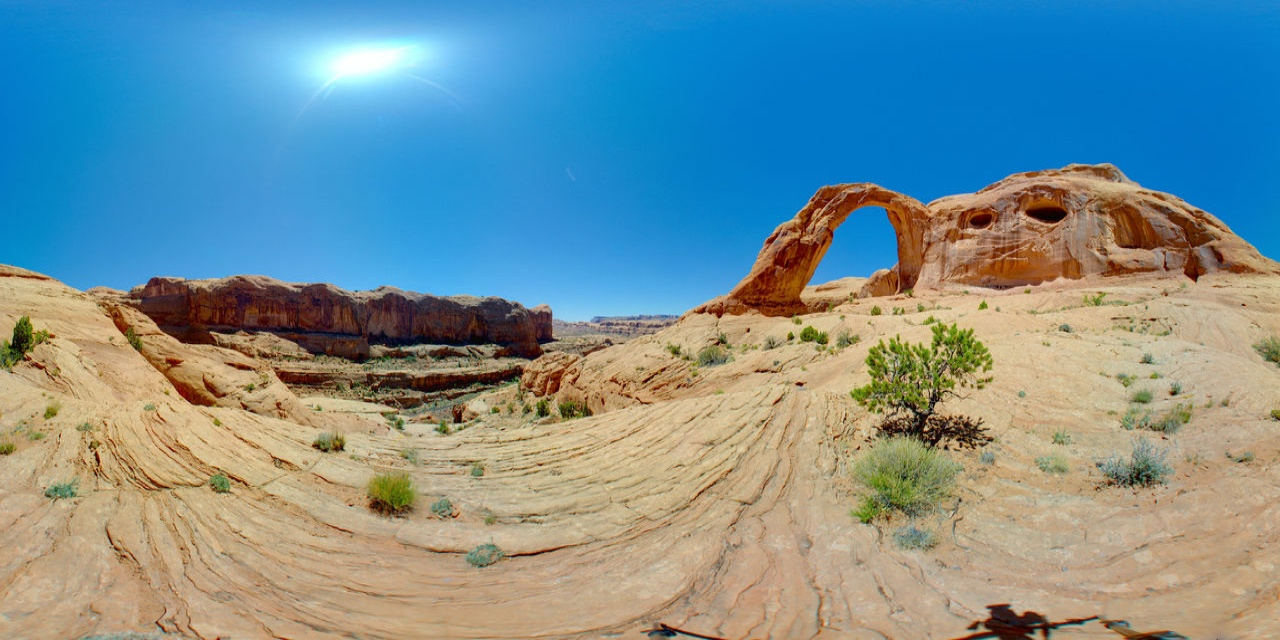
\includegraphics[width=1\textwidth]{img/image (9).jpg}
        \caption{Outdoor equirectangular image.}
        \label{subfig:out_equi}
    \end{subfigure}\hfill
    \begin{subfigure}{0.47\linewidth}
        \centering
        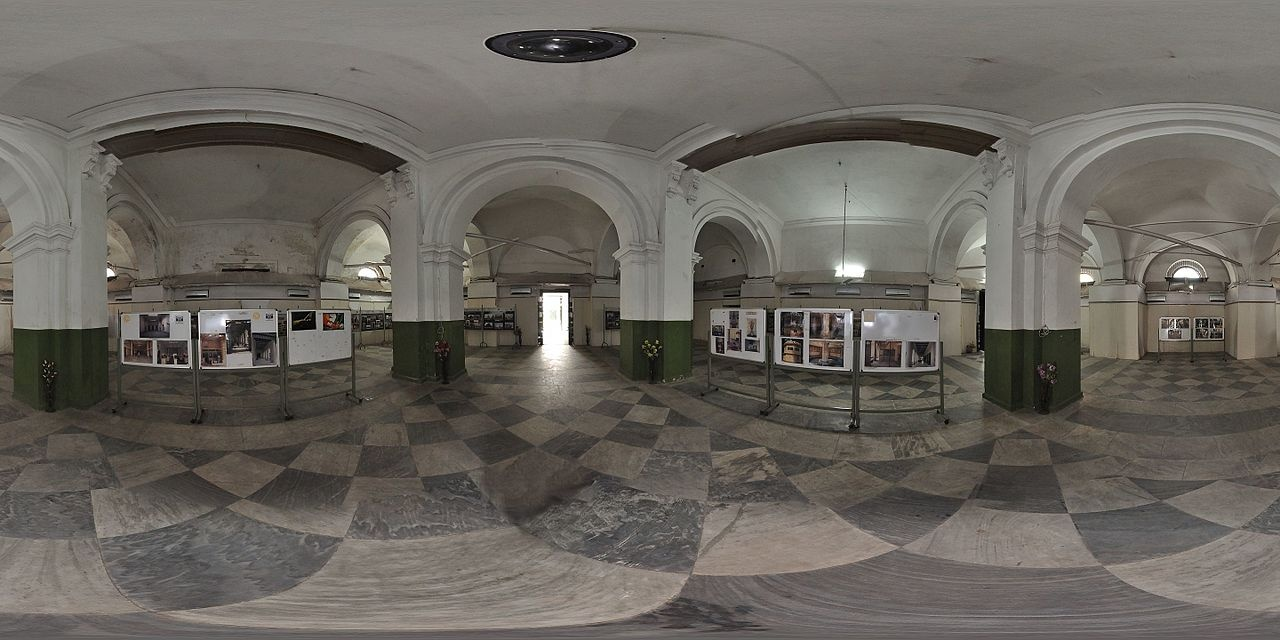
\includegraphics[width=1\textwidth]{img/image (10).JPG}
        \caption{Indoor equirectangular image.}
        \label{subfig:in_equi}
    \end{subfigure}

\caption{Examples of 360° scenes represented through equirectangular projection.}
\label{fig:equirectangular_proj}
\end{figure}

The remainder of this dissertation proposal is structured as follows. Section~\ref{sec:subtitles} presents current solutions for subtitles positioning in 360º video. Section~\ref{sec:approach} details our proposed approach for automatic subtitles positioning. In Section~\ref{sec_4}, we present the contributions we already achieved in this work. Section~\ref{sec_5} contains the remaining contributions we expect to achieve by the end of this research. Finally, in Section~\ref{sec_6}\ we present our schedule.



\section{Approach}
\label{sec:approach}
Let us define as \emph{actor} each person present in a 360º video. Therefore, the goal of our approach is to place subtitles based on the actors' position on a given 360° video. To accomplish this goal, we use face detection and clustering mechanisms to identify the actors' trajectory in 360° video. Then, based on this trajectory, we place dynamic subtitles following the actors' path. For dicdatic purposes, we decided to divide our exposition in three phases: (i)~\emph{face detection in 360° videos}, (ii)~\emph{actors clusterization}, and (iii)~\emph{dynamic subtitles positioning}. These phases are described in the following subsections. 

\subsection{Face Detection in 360° videos}

In this phase, we aim at detecting the actors' faces present in the 360° video frames using object detection models.
%%
In general, an object detection model can identify which, among a known set of objects, are present in the image, and provides information about their positions with bounding boxes.
%%
Bounding boxes are specified by the $x$ and $y$ axes coordinates of the upper-left corner and of the lower-right corner of the rectangle that establishes the visual limits that encapsulate each object.
%%
In our case, objects are faces and, therefore, the face detection model is responsible for returning the position of the faces in an image~(video frame).
%%

Because of the distortions present on the equirectangular projection, we opted for elaborating a solution based on viewports extraction. A viewport is defined by its center, in polar coordinates~(lat, long), and its field of view~(FoV). Figure \ref{fig:viewports} shows viewports extracted at different polar coordinates from Figure \ref{subfig:out_equi}.

\begin{figure}[!ht]
    \centering
    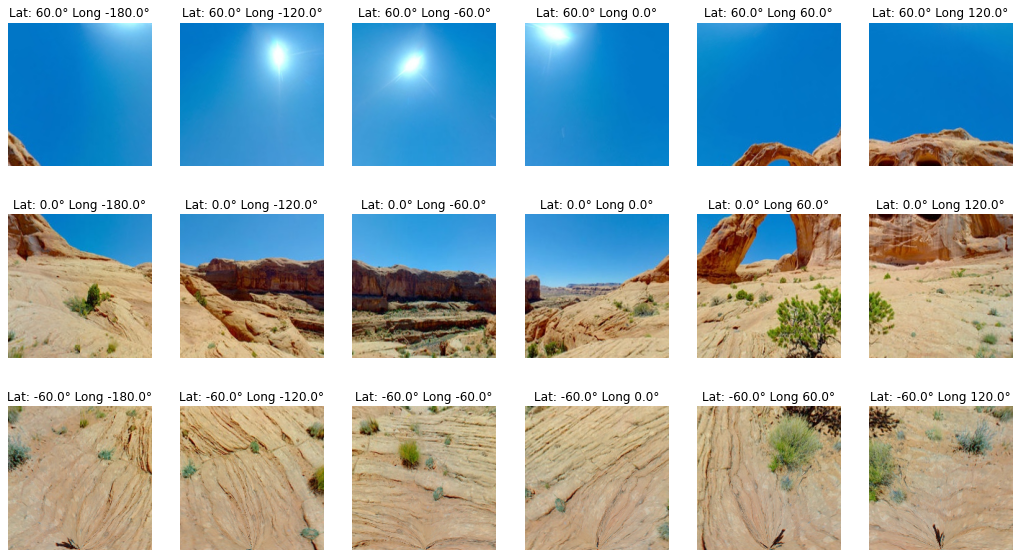
\includegraphics[width=1\textwidth]{img/viewports.png}
    \caption{Viewports extracted at different polar coordinates with $FoV = 60^{\circ}$}
    \label{fig:viewports}
\end{figure}

For each viewport, we apply a face detection model. 
Then, we project the faces detected bounding boxes back to the equirectangular image. For doing that for a given bounding box, we project the four corners and the mean point of each edge~(8 points in total). Therefore, in the equirectangular image, we deal with polygons instead of bounding boxes, due to the distortions introduced. As different viewports may intersect and cover part of the same region in an image, we apply Non-maximum Supression~(NMS), eliminating intersected detections within a given threshold. One of the main advantages of this approach is that we can use face detection models trained in regular images, since distortions are reduced with the use of viewports.

Due to the lack of datasets for face detection in equirectangular images, we created a synthetic dataset based on the FDDB dataset~\cite{fddbTech}, a popular benchmark for face detection evaluation containing 2845 images and 5171 faces. We collected 19 indoor and outdoor equirectangular images, from Google Images,\footnote{https://www.google.com/imghp} ESO,\footnote{https://www.eso.org/public} and PxHere.\footnote{https://pxhere.com}
For each image in the FDDB dataset, we randomly chose a latitude, longitude and equirectangular image to project it. For each face present on that image, we projected the bounding box to a polygon exactly as mentioned in the viewport process. Figure \ref{fig:fddb_proj} shows an example of an image from FDDB projected in the polar coordinates \emph{lat} $ = -60^{\circ}$ \emph{long} $= 0^{\circ}$ to an equirectangular image.

\begin{figure}[!ht]
\centering
    \begin{subfigure}{0.4\linewidth}
        \centering
        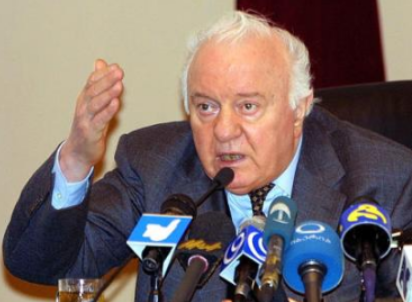
\includegraphics[height=10em]{img/face_pre.png}
        \caption{FDDB image example.}
        \label{subfig:face_pre}
    \end{subfigure}\hfill
    \begin{subfigure}{0.55\linewidth}
        \centering
        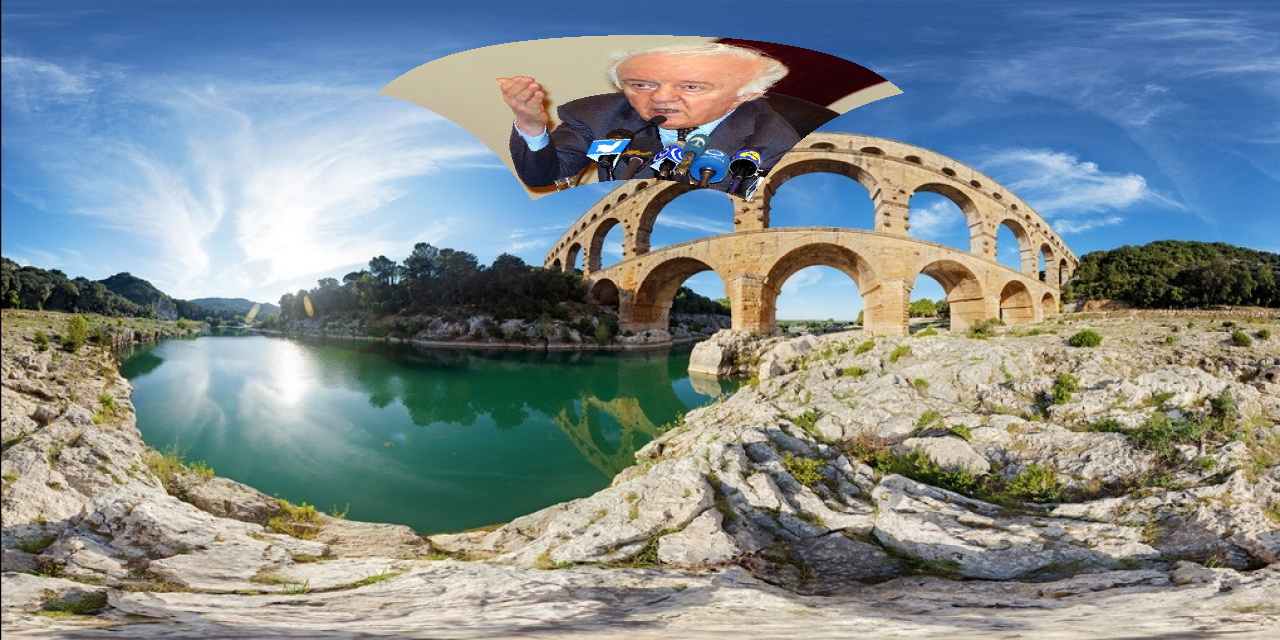
\includegraphics[height=10em]{img/face_pos.png}
        \caption{Projection example of FDDB image.}
        \label{subfig:face_pos}
    \end{subfigure}

\caption{FDDB image projection to Equirectangular image.}
\label{fig:fddb_proj}
\end{figure}

As evaluation metric, we use Mean Average Precision~(mAP), that is commonly used to evaluate object detection algorithms~[ref]. As face detector, we implemented a solution using MTCNN~\cite{mtcnn} (Multitask Cascaded Convolutional Networks) which is widely used for the face detection task~\cite{mtcnn1, mtcnn2, mtcnn3}. %If we have time, we also intend to test YOLO

In summary, for this phase, we have defined the following tasks:

\begin{itemize}
    \item \textbf{T 1.1}: Implementation of model based on viewports for face detection in 360° equirectangular images~(100\% complete).
    \item \textbf{T 1.2}: Synthetic dataset creation~(100\% complete).
    \item \textbf{T 1.3}: Model test in the dataset using MTCNN and MTCNN with viewports~(100\% complete).
    \item \textbf{T 1.4}: Results evaluation using mAP~(100\% complete).
\end{itemize}


\subsection{Actors Clustering}

The main objective of this phase is to group the actors present in different frames of a given 360° video, so that we can track the trajectory of such actors throughout the duration of the video. 

For each face detected in the previous phase, we generate embeddings that represent it.
%%
The objective of the embeddings generation step is to represent each face image as a vector space in $\mathbb{R}^{n}$.
%%
To achieve that, it processes each of the faces generated in the previous phase through a Convolutional Neural Network~(CNN), generating embeddings. 
%%
An embedding is a representation of the input in a lower dimensionality space.
%%
Ideally, an embedding captures some semantics of the input, e.g. by placing semantically similar inputs close together in the embedding space.
%
At the end of this step, we have all faces represented as embeddings.
%%

Once we have all the faces from all frames represented as embedding, we group such embeddings and, consequently, faces that are close in the embedding space using a clustering algorithm. 
%
Clustering is the task of dividing a set of data points, embeddings in this case, into a number of groups~(clusters) such that data points in a given group are similar to other data points in the same group and dissimilar to the data points in other groups.
%%
The clustering process should produce a partition of the dataset, i.e., each generated cluster represents a specific person, and the union of all clusters covers the whole dataset.

In \cite{mendes2020cluster}, we collected a dataset using the information provided by the Brazilian Chamber of Deputies\footnote{\url{https://www.camara.leg.br/}} for the 55th legislature, which was in session from February 1st, 2015 through January 31st, 2019.
%%
In total, 623 different deputies participated during some period in the 55th legislature, but we collected only 513 deputies from this set.
%%
For each of the 513 deputies, we collected images in which he/she was present using Google Images.
%%
The resulting dataset had a total of 9,003 images, with a mean of ~17.55 images per deputy and a standard deviation of ~6.91. 
%%
The maximum and minimum number of images per deputy are respectively 32 and 2.
%%
We have randomly selected one image of each deputy for validation and the rest for training.
%%
Thus, our dataset was divided in two: the training set, with 8,490 images, and the validation set, with 513 images.  
%%
We tested three different CNNs for the \emph{Embeddings Generation} step in association with three different clustering algorithms for the \emph{Clustering} step.
%%
For that, we evaluated each pair of \emph{CNN x ClusteringAlg} through the quality of the clusters they generated. 
%%
To experiment, we used the training set with 8490 deputy images.

For embeddings generation, we had three candidate CNNs that were previously trained on the VGGFace2 dataset~\cite{cao2018vggface2}. 
%%
The VGGFace2 dataset contains $3.31$ million images of $9131$ subjects and has large variations in pose, age, illumination, ethnicity, and profession.
%%
The three candidate CNNs used are VGG-16~\cite{vgg16}, ResNet-50~\cite{resnet} and SE-ResNet-50~\cite{senet}~(SeNet-50 for short). VGG-16 generates embeddings in the $\mathbb{R}^{512}$  feature space, while ResNet-50 and SeNet-50 generate embeddings in the $\mathbb{R}^{2048}$ feature space.  
For clustering, we selected the following clustering algorithms as candidates: k-Means \cite{lloyd1982least}, affinity propagation \cite{frey2007clustering}, and agglomerative clustering \cite{ward1963hierarchical}.


We evaluated each combination~(\emph{CNN x ClusteringAlg}) using the V-Measure \cite{vmeasure}, which is an entropy-based measure that computes how successfully the criteria of homogeneity and completeness have been satisfied. This metric is extensively used for comparing clustering solutions and has been used in different domain fields such as biology \cite{bio1}, computational linguistics \cite{nlp1}, and document engineering \cite{doceng}.

\begin{table}[!ht]
%\vspace{-1em}
\centering
\small
\caption{Results of the evaluation of the clusters created by each combination of CNN and clustering algorithms.}
\begin{tabular}{@{}ccccc@{}}
\toprule
\textbf{CNN} & \textbf{Clustering} & \textbf{$h$} & \textbf{$c$} & \textbf{$V_1$} \\ \midrule
                  & KM                  & 0.9665                     & 0.9675                      & 0.9670             \\
ResNet-50         & AP                  & 0.0000                     & 1.0000                      & 0.0000             \\
                  & AC                  & 0.9821                     & 0.9798                      & 0.9810             \\ \midrule
                  & KM                  & 0.9725                     & 0.9726                      & 0.9725             \\
SeNet-50          & AP                  & 0.9859                     & 0.9558                      & 0.9706             \\
                  & \textbf{AC}         & \textbf{0.9862}            & \textbf{0.9833}             & \textbf{0.9847}    \\ \midrule
                  & KM                  & 0.8340                     & 0.8415                      & 0.8378             \\
VGG-16            & AP                  & 0.0000                     & 1.0000                      & 0.0000             \\
                  & AC                  & 0.8899                     & 0.8929                      & 0.8914             \\
\end{tabular}
\label{tab:results_clustering}
\vspace{-1em}
\end{table}

From Table \ref{tab:results_clustering}, we concluded that the best combination of CNN and clustering algorithm was SeNet-50 with Agglomerative Clustering. Then, we used this combination in thirteen videos, being able to track the actors in them. Figure \ref{fig:timeline1} shows the actors present in one of the videos with the frames tagged with colors representing the actors present on them.

\begin{figure}[!ht]
    \centering
    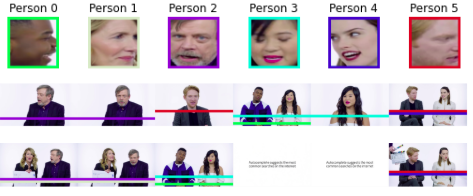
\includegraphics[width=0.7\textwidth]{img/timeline2.png}
    \caption{Timeline with tagged frames by their clusters~(actors) present.}
    \label{fig:timeline1}
\end{figure}


%%%%%%%%%%%%%%%%%%%%%%%%%%% ism

Following this approach, in \cite{mendes2020ISM}, we used actors face clustering for recommending videos that share the presence of the same actors. As we obtained the best results with the combination SeNet-50 with Agglomerative Clustering in \cite{mendes2020cluster}, we used this same combination in \cite{mendes2020ISM}. 
In that work, we used actors face clustering in 98 videos and around 72\% of the faces went to the correct clusters. Figure \ref{fig:timeline2} shows part of the timeline of one of the videos tagged with colors representing the color of each actor present.

\begin{figure}[!ht]
    \centering
    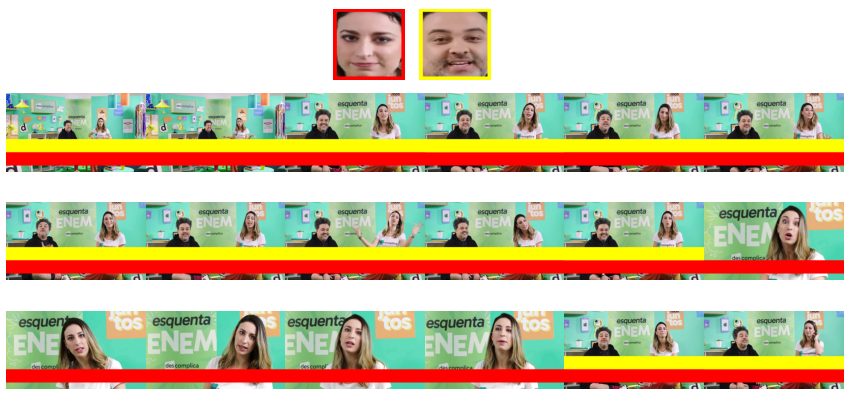
\includegraphics[width=0.75\textwidth]{img/educational_timeline2.png}
    \caption{Timeline with tagged frames by their clusters~(actors) present.}
    \label{fig:timeline2}
\end{figure}

Due to the distortions present in 360° video frames, we return the faces detected in the viewports to pass through the embeddings generation and clustering steps. By doing so, the possible distortions present in the face detected are reduced. We expect that, in the end of this phase we will have, for a given 360° video, the trajectory of each actor throughout the duration of the video.

In summary, for this phase, we have defined the following tasks:


\begin{itemize}
    \item \textbf{T 2.1}: Evaluation of combinations of CNNs and clustering algorithms~(100\% complete).
    \item \textbf{T 2.2}: Evaluation of faces clustering with videos~(100\% complete).
    \item \textbf{T 2.3}: Development of a method to correct distortions before faces clustering in 360° video~(100\% complete).
\end{itemize}


\subsection{ML-Based Dynamic Subtitles Positioning}

The main objective of this phase is to position subtitles considering the position of the actors in the 360° video.

In \cite{mendes_2020}, we proposed a model for authoring interactive 360° video. In such a model, we can define interactive 360° video that are presented together with additional information attached to it, such as image, text and spatial audio. The positioning of such additional information is defined by their polar coordinates, start time and duration. Moreover, we can also configure behaviours depending on where the user is looking. For instance, we can define that a text moves with the user's head motion and is always visible or that such text is placed at fixed position if it is in the field of view of the user. Besides the design of such a model, we developed a player that follows the definitions of our model and is able to play interactive 360° video defined by it. Then, we can use the results obtained from the previous phases to define the positioning of subtitles according to the actors positioning using our player.

For testing our approach, we intend to select 360º video with people present and talking as case studies so that we can verify the applicability of our solution. Our strategy fits in the category described in Section \ref{subsubsec:speaker_following}, but different from the strategies presented there, ours use machine learning to help content creators define how subtitles behave.

In summary, for this phase, we have defined the following tasks:

\begin{itemize}
    \item \textbf{T 3.1}: Definition of a model that supports subtitles positioning using polar coordinates~(100\% complete).
    \item \textbf{T 3.2}: Development of a player that supports dynamic subtitles positioning depending on the users' field of view~(100\% complete).
    \item \textbf{T 3.3}: Selection and development of interactive 360º videos with dynamic subtitles. (20\%)
\end{itemize}

\section{Contributions}
\label{sec_4}
 As collateral contributions of this research, three papers have been published in relevant multimedia conferences \cite{mendes2020cluster, mendes_2020, mendes2020ISM}. In \cite{mendes_2020}, we have developed an authoring model and a player for interactive 360º video. In \cite{mendes2020cluster}, we have evaluated video face clustering together with a cluster-matching method for video face recognition. In \cite{mendes2020ISM}, we have used video face clustering and the presence of actors in different video as a mean for recommending educational videos. We have also created a synthetic dataset for face detection in equirectangular images.

\section{Expected Contributions}
\label{sec_5}
In this dissertation proposal we have proposed an ML-based solution for face clustering and subtitles positioning in 360° video. We expect that our method together with our authoring model and player will help content creators in the process of authoring interactive 360-degree video with subtitles.


\section{Schedule}
\label{sec_6}
Table \ref{tab:schedule} presents the schedule we propose for completing the remainder tasks of this research.

\definecolor{darkgray}{RGB}{180,180,180}
\definecolor{gray}{RGB}{205,205,205}
\definecolor{lightgray}{RGB}{218,218,218}
\definecolor{lightlightgray}{RGB}{238,238,238}

\definecolor{darkred}{RGB}{204,0,0}
\definecolor{red}{RGB}{224,102,102}
\definecolor{lightred}{RGB}{244,199,195}

\definecolor{darkmagenta}{RGB}{61,133,198}
\definecolor{magenta}{RGB}{111,168,220}
\definecolor{lightmagenta}{RGB}{166,206,242}

% \definecolor{mark}{RGB}{224,102,102} %red
\definecolor{mark}{RGB}{111,168,220} %magenta

\definecolor{white}{RGB}{255,255,255}

\arrayrulecolor{white}
% \arrayrulecolor{darkgray}
\setlength\tabcolsep{3.0pt} % space between the text and the left/right border. Default Value = 6.0pt

\begin{table} [!ht]
  \centering
  \caption{Schedule of this dissertation proposal.}
  \label{tab:schedule}

  \begin{tabularx}{21em}{|p{6em}|p{5em}|p{5em}|p{5em}}
 
  \rowcolor{darkgray} & 
  \multicolumn{3}{|c|}{\textbf{2021}}\\ 
  
  \rowcolor{gray}
  \multicolumn{1}{|c|}{\multirow{-2}{*}{\cellcolor{darkgray}\textbf{Tasks}}} & 
  \multicolumn{1}{|c|}{\textbf{May}} & 
  \multicolumn{1}{|c|}{\textbf{Jun}} & 
  \multicolumn{1}{|c|}{\textbf{Jul}}\\
%   \hline
%%%%%%%%%%%%%%%%%%%%%%%%%%%%%%%%%%%%%%%%%%%%%%%%%%%%%%%%%%%%%%%%%%%%%%%%%%%%%%%%%%%%%%%%%%%%%%%%%%%%%%%%%%%%%%%%%%%%%%%%%%%%%%%%%%%%%%
  \rowcolor{lightgray}
       & \cellcolor{mark} &  &\\
  \rowcolor{lightgray}
    \multicolumn{1}{|c|}{\multirow{-1}{*}{T1}}
       & \cellcolor{mark} & &\\
  \rowcolor{lightgray}  
   & \cellcolor{mark} & & \\
%   \hline
%%%%%%%%%%%%%%%%%%%%%%%%%%%%%%%%%%%%%%%%%%%%%%%%%%%%%%%%%%%%%%%%%%%%%%%%%%%%%%%%%%%%%%%%%%%%%%%%%%%%%%%%%%%%%%%%%%%%%%%%%%%%%%%%%%%%%%
  \rowcolor{lightlightgray}
  &  & \cellcolor{mark}  & \cellcolor{mark}\\
  \rowcolor{lightlightgray}
    \multirow{-2}{*}{Dissertation} 
    &  & \cellcolor{mark}  & \cellcolor{mark}\\
  \rowcolor{lightlightgray}
    \multirow{-2}{*}{Writing} 
    &  & \cellcolor{mark}  & \cellcolor{mark}\\
%   \hline
%%%%%%%%%%%%%%%%%%%%%%%%%%%%%%%%%%%%%%%%%%%%%%%%%%%%%%%%%%%%%%%%%%%%%%%%%%%%%%%%%%%%%%%%%%%%%%%%%%%%%%%%%%%%%%%%%%%%%%%%%%%%%%%%%%%%%%
  \rowcolor{lightgray}
  &  &  & \cellcolor{mark}\\
  \rowcolor{lightgray}
    \multirow{-2}{*}{Dissertation} 
  &  &  & \cellcolor{mark}\\
  \rowcolor{lightgray}
  \multirow{-2}{*}{Presentation}
  &  &  & \cellcolor{mark}\\
\arrayrulecolor{darkgray}    

%   \end{tabular}
  \end{tabularx}
\end{table}

% Development of model instantiation
% Preliminary evaluation 
% Evaluation 
% Evaluation data analysis
% Thesis writing
% Thesis defense